\section{Métrica y modelado de la confiabilidad de sistemas}\label{sec:metrica_modelado}
Es de suma importancia llevar a cabo el análisis de la confiabilidad, disponibilidad y mantenibilidad (RAM\footnote{Del ingles, Realibility, Availability, Maintainability}) de sistemas satelitales, durante la fase de diseño \citep{Hoque15}, a fin de lograr la mínima cantidad de fallas o incrementar el \ac{MTBF} \citep{Peng13}. Llevar esto a cabo es fundamental, ya que permite el desarrollo de estrategias que facilitan altos grados de confiabilidad, disponibilidad y mantenibilidad \citep{Hoque15}.

Existen dos categorías de medición de la confiabilidad y predición, estas son utilizadas para asegurar la seguridad del software de sistemas críticos \citep{Schneidewind97}, las cuales son:
  \begin{itemize}
    \item medición y predicción que están asociadas con las fallas y errores residuales.
    \item medición y predicción que están asociadas con la disponibilidad del sistema a sobrevivir durante la misión sin experimentar fallas
      (o pérdidas) en el sistema.
  \end{itemize}

  Las dos categorías mencionadas anteriormente son explicadas en \cite{Schneidewind97}.

  Según \cite{Liu14} las severidades de las fallas son clasificadas como críticas, peligrosas o triviales, teniendo en cuenta la contribución de esa falla a la pérdida de la misión. Es importante, además, conocer el riesgo de una falla. El riesgo, se define como la posibilidad de que una falla produzca una lesión (por ejemplo, un astronauta en vuelos tripulados), algún daño material (por ejemplo, la destrucción del satélite), o una pérdida (por ejemplo, la pérdida de la misión).

  Dependiendo de la misión, un criterio para definir si un sistema es seguro o no, es reduciendo las fallas que pueden provocar pérdidas de vida, de la misión o la obligación de abortar una misión \citep{Schneidewind97}. \cite{Schneidewind97} define dos criterios que deben satisfacerse:
  \begin{itemize}
    \item $r(t_t) < r_c$,
    \item $T_F(t_t) > t_m$
  \end{itemize}

  dónde $t_t$ es el Tiempo total de testing (observado o predicho); $r(t_t)$ son las fallas restantes hasta $t_t$; $r_c$ es una valor crítico de fallas restantes; $T_F(t_t)$ es la métrica para medir el riesgo; y $t_m$ es la duración de la misión.

  Lo anterior significa que un sistema crítico será seguro si: las fallas restantes en el tiempo de prueba son menores a un valor crítico de cantidad de fallas, o la duración de una misión es menor al tiempo que se de la siguiente falla.
  
  En la literatura se utilizan modelos matemáticos para modelar los sistemas críticos y calcular así su confiabilidad. La mayoría de ellos asumen, que todas las fallas tienen igual tasa de detección de fallas, como así también la misma severidad, lo cual no es correcto \citep{Liu14}. Las técnicas de verificación formal tienen un fuerte enfoque para la verificación tanto de sistemas complejos, como de las propiedades deseadas de los sistemas \citep{Peng13}. Es importante llevar a cabo una verificación de modelo\footnote{Model checking}, esta incluye técnicas de verificación automática para sistemas de estados concurrentes finitos. En estos modelos, las especificaciones de los sistemas son escritos en una lógica temporal y proposicional, y el procedimiento de verificación es una búsqueda del espacio de estado del diseño \citep{Hoque15}.

  En \cite{Hoque15} se utiliza la \textit{verificación probabilística de modelos}, la cual es utilizada para verificar sistemas, de los cuales los comportamientos son estocástico por naturaleza. Este se basa en la construcción y análisis de modelos probabilísticos como cadenas de Markov. En \cite{Hoque15} se indica que estas técnicas fueron aplicadas en misiones de \ac{NASA}. Los modelos de Markov son muy utilizados para los análisis de confiabilidad y disponibilidad de sistemas complejos \citep{Hoque15}.

  En \cite{Hoque15} se lleva a cabo un modelo simplificado de un sistema satelital el cual se muestra en la Figura \ref{fig:SystemSatellite}. La descripción del modelo se llevó a cabo usando el lenguaje PRISM. El modelo que se describe en \cite{Hoque15} y \cite{Peng13} se refiere a un modelo a nivel de sistema/misión, muy diferente a lo que se pretende realizar en este trabajo de tesis, pero es factible basarse en los conceptos que describe la literatura, ya que lograron aumentar la confiabilidad del modelo propuesto, en contraposición de modelos ``clásicos''.

\begin{figure}[H]
  \centering
  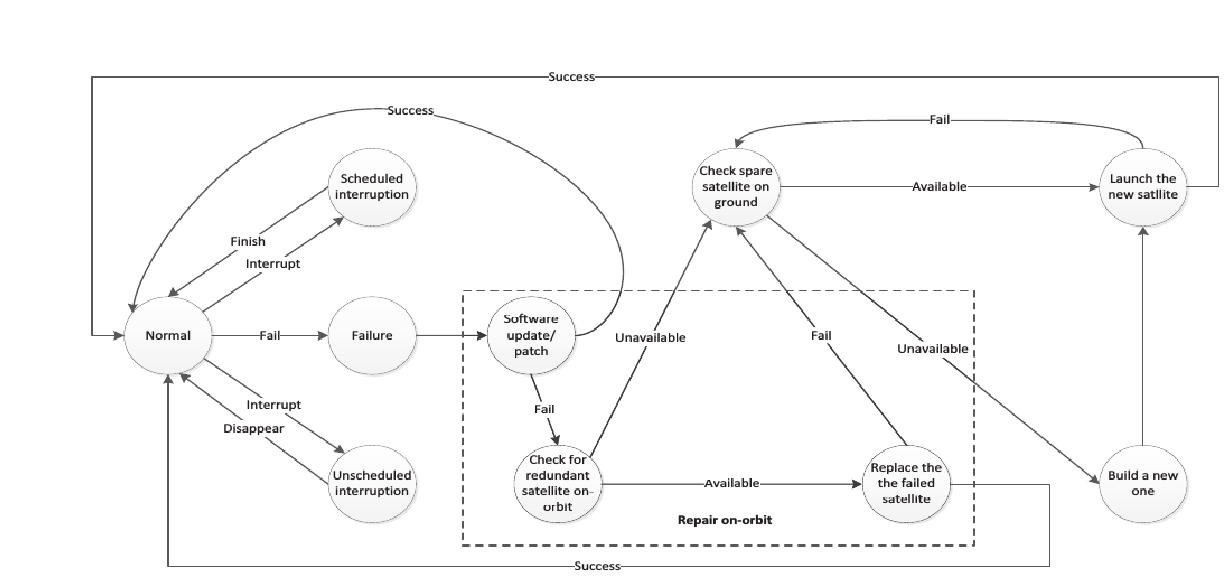
\includegraphics[scale=0.4]{images/Marco_teorico/SatelliteSystemModel.png}
  \caption{Modelo de sistema satelital \citep{Hoque15}}  
  \label{fig:SystemSatellite} 
\end{figure}

\cite{Hoque15} y \cite{Peng13} relacionan tasa de falla $\lambda$, confiabilidad $R_e$ y \ac{MTBF} con la siguiente ecuación $$\lambda = \frac{-ln R_e}{MTBF}$$

\cite{Esteve12} muestra el caso de estudio del desarrollo de una plataforma satelital a un alto nivel conceptual. Demuestran la correcta utilización de métodos formales y herramientas para la industria satelital. Se utiliza la herramienta desarrollada por el consorcio COMPASS\footnote{Correctness, Modeling and Performance of Aerospace Systems} para el modelado formal y análisis, que es utilizado por la industria espacial de Europa. Llegan a la conclusión de que mediante la utilización de modelos formales, se logra desarrollar un modelo completo, que cumple con todos los aspectos necesarios. Esto asegura la consistencia de los análisis \citep{Esteve12}.

El estado de la cuestión sobre la temática tratada en esta sección, indica que debería utilizarse modelos formales para el análisis de los sistemas. Se llega a la conclusión de que no existe un método (o modelo) completo y exclusivo para lo que se pretende desarrollar en este trabajo de tesis. Por ello se deberá utilizar y moldear las metodolgías vistas en esta sección, para lograr cumplir con los obejetivos del presente trabajo. 


